% Diagrama de secuencia editable. Los objetos anónimos usan el prefijo ':'.
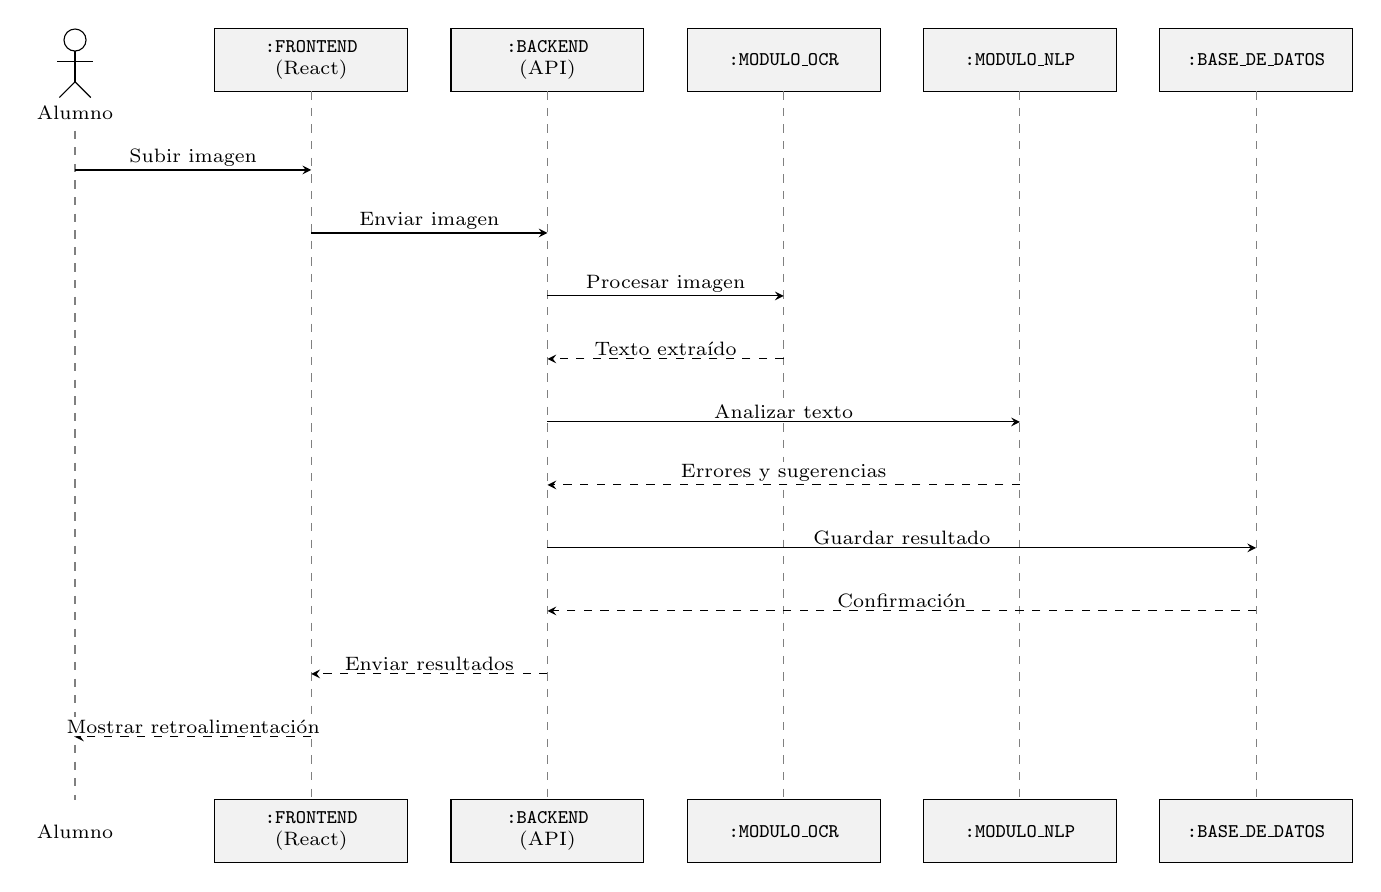
\begin{tikzpicture}[
  participante/.style={draw,fill=gray!10,minimum width=2.45cm,minimum height=0.8cm,align=center,font=\scriptsize},
  mensaje/.style={font=\scriptsize,fill=white,inner sep=1pt},
  linea/.style={dashed,gray},
  llamada/.style={->,>=stealth},
  respuesta/.style={->,>=stealth,dashed}
]
\draw (0,0.25) circle (0.14);
\draw (0,0.11)--(0,-0.28) (0,-0.02)--(-0.23,-0.02) (0,-0.02)--(0.23,-0.02);
\draw (0,-0.28)--(-0.2,-0.48) (0,-0.28)--(0.2,-0.48);
\node[font=\scriptsize] at (0,-0.68) {Alumno};
\node[participante] at (3,0) {\texttt{:FRONTEND}\\(React)};
\node[participante] at (6,0) {\texttt{:BACKEND}\\(API)};
\node[participante] at (9,0) {\texttt{:MODULO\_OCR}};
\node[participante] at (12,0) {\texttt{:MODULO\_NLP}};
\node[participante] at (15,0) {\texttt{:BASE\_DE\_DATOS}};
\draw[linea] (0,-0.9)--(0,-9.4);
\foreach \x in {3,6,9,12,15} {\draw[linea] (\x,-0.4)--(\x,-9.4);}
\draw[llamada] (0,-1.4)--node[mensaje,above]{Subir imagen}(3,-1.4);
\draw[llamada] (3,-2.2)--node[mensaje,above]{Enviar imagen}(6,-2.2);
\draw[llamada] (6,-3.0)--node[mensaje,above]{Procesar imagen}(9,-3.0);
\draw[respuesta] (9,-3.8)--node[mensaje,above]{Texto extraído}(6,-3.8);
\draw[llamada] (6,-4.6)--node[mensaje,above]{Analizar texto}(12,-4.6);
\draw[respuesta] (12,-5.4)--node[mensaje,above]{Errores y sugerencias}(6,-5.4);
\draw[llamada] (6,-6.2)--node[mensaje,above]{Guardar resultado}(15,-6.2);
\draw[respuesta] (15,-7.0)--node[mensaje,above]{Confirmación}(6,-7.0);
\draw[respuesta] (6,-7.8)--node[mensaje,above]{Enviar resultados}(3,-7.8);
\draw[respuesta] (3,-8.6)--node[mensaje,above]{Mostrar retroalimentación}(0,-8.6);
\node[font=\scriptsize] at (0,-9.8) {Alumno};
\node[participante] at (3,-9.8) {\texttt{:FRONTEND}\\(React)};
\node[participante] at (6,-9.8) {\texttt{:BACKEND}\\(API)};
\node[participante] at (9,-9.8) {\texttt{:MODULO\_OCR}};
\node[participante] at (12,-9.8) {\texttt{:MODULO\_NLP}};
\node[participante] at (15,-9.8) {\texttt{:BASE\_DE\_DATOS}};
\end{tikzpicture}
